\chapter{Introduction}\label{chap:introduction}
% \section{Introduction}
% 2 pages
   \begin{figure}[!ht]
        \centering
        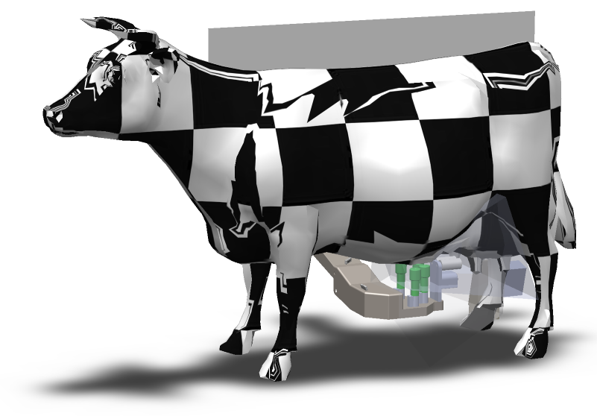
\includegraphics[width=0.7\textwidth]{images/cow_system.png}
        \caption{3D Prototype Model of the Cow Milking Robot}
        \label{fig:cow_fmc}
    \end{figure}
    
\section{Use Case: Improving the Cow Milking Automation}\label{chap:3:use-case}

Current international state of the art
Milking robots have been used successfully in agriculture for over 20 years. However, the concepts of the dominant systems available on the market have hardly been adapted to the latest technical developments during this time. For example, at the largest supplier Lely, most of the drives are still electro-pneumatic spindle motors even in the latest version of the milking robot (type Astronaut A5). The reason is the lower price, as well as the inherent compliance of these drives, which makes it easy to implement protection of the robot mechanics against cow kicks. However, these electro-pneumatic drives require a lot of maintenance. In particular, the seals of these drives must be replaced regularly so that the robot system remains operational. This drive solution thus also often leads to unplanned downtime of the milking robot.
In Swiss farms, the herd size is in many cases such that more than one milking system is needed, but the two milking robots required for this have no space in the existing barn. Thus, a costly conversion or even a new construction of the barn is necessary.

In order to bring the teat cups to the teats with the robot, the position of the cow and the exact position of the teats must be recorded. The current milking robots mostly use 2D laser scanners for this purpose. The acquisition is static, i.e. the robot does not move during a measurement process. In order to create a 3D image with 2D scans, from which the position of the teats can be determined, several measurements are necessary. This takes a lot of time, and if the cow moves during the measurement, the measurement process even has to be restarted.

Novelty of the technology of a modern milking robot

For the new milking robot to be developed in this project, only electric drives will be used. Modern electric drives are now much cheaper than they were 20 years ago, so their cost disadvantage compared to electro-pneumatic drives is no longer great. Electric drives can also be controlled much more precisely. With suitable control strategies, robot compliance can also be achieved with electric drives. The greatest advantage of electric drives, however, is that they can be operated practically maintenance-free if suitably designed, resulting in a much more reliable system with higher availability.
    
Furthermore, a much more compact kinematic structure is to be selected for the robot arm that guides the teat cups to the teats, for example similar to that of Scara robots. A major advantage of the new overall concept is that, unlike competitor models, two or more manipulators can be operated on one basic system (pump, cooling, storage). This means that the overall system can be designed smaller and thus, in many cases, can be installed in already existing barn structures. In addition, such a system can be realized more cost-effectively. SLG has already filed a patent to protect this concept (REFERENCE).

Another novelty of the new milking robot can be found in the field of sensor technology to detect the position of the teats. In recent years, several new and very inexpensive 3D cameras have been introduced to the market that can be used to detect the position of the teats. These cameras directly generate 3D point clouds with high resolution at measurement rates of up to 30 frames/s. With these sensors, the position of the teats can be captured dynamically, i.e. directly during the movement of the robot or the teat cups to the teats. The 3D measurements must be calculated in real time with the current position of the robot. 

Although this requires much more complex data processing on a powerful control system, it does away with a time-consuming, separate 
time-consuming, separate measurement process can be dispensed with. Dynamic measurement with modern sensors also offers the potential to be much more robust and reliable than the measurement methods used today.
    
    % \begin{itemize}
    %     \item describe the general need for automated cow milking
    %     \item describe how the problem is currently being solved briefly
    
    %     \item describe the challenges in cow teat recognition: morphology/shapes and movement
    %     \item describe how these methods fail || describe challenges/limitations of current methods (sensors, etc, no memory)
    
    %     \item can solve this problem with computer vision briefly
    
    %     \item describe cow project main driver (The InIT's purpose) (do we mention how expensive current solutions are?)

    % \end{itemize}
\section{Towards 3D Object Detection}\label{chap:1:detection}
\lipsum[2-5]

    % \begin{itemize}
    %     \item describe advancements in traditional computer vision for image interpretation
    %     \item list shortcomings/challenges we can overcome with computer vision
        
    %     \item describe advancements in computer vision with DL for object detection
    %     \item list shortcomings/challenges we can overcome with computer vision
        
    %     \item shortcoming1: no object permanence | objects out of sight
    %     \item shortcoming2: reliability of only detecting cow teats (?)
    %     \item HELP: shortcoming3: (?) (need to re-read the papers from gio)

    % \end{itemize}
\section{Problem Description}\label{chap:1:problem}
% \lipsum[2-3]
Sutter Landtechnik GmbH (SLG) in Andwil SG and Muolen SG offers sales, installation and service of technical equipment and machinery for various tasks in agriculture. The customers are farms of various sizes in German-speaking Switzerland and in nearby foreign countries. In addition to the areas of tractors and agricultural technology (e.g. harvesting machines), farm technology (barn equipment), there is the area of milking technology, which, in addition to milking machines, includes cooling technology and, last but not least, milking robots. Various machines, including milking technology, were developed by SLG itself and are also manufactured in its own plant. Of the approximately 50,000 farms in Switzerland, about 2,000 are customers of SLG. In addition, there are about 200 farms from nearby foreign countries. With these, SLG generates an annual turnover of ~6.3 MCHF (2018) with its 25 employees. All milking robot systems installed and/or maintained by SLG are of the "Astronaut" type from the Dutch company Lely.

The Lely company with the Astronaut model range has been able to establish itself on the European market for a variety of reasons and is by far the market leader. The European market is dominated by two brands, Lely 55% and DeLaval 30% of the market. In Switzerland

there are currently around 850 Lely Astronaut and around 300 DeLaval VMS milking robots in operation. The Swiss market is clearly dominated by Lely with a market share of about 72%. The weak competition, as well as the small Swiss market in relation to Europe, means that specific adaptations only for the Swiss market are not worthwhile for the large groups.

In recent years, the financial pressure on agriculture in Switzerland has increased massively. Since 1980, the number of farms has been shrinking by about 1000 farms per year. The Swiss consumer wants more and more organically grown products and at the same time consumer prices are getting cheaper and cheaper. The extensive Swiss animal welfare regulations, which are the strictest in Europe, make animal husbandry even more expensive. All this leads to the fact that the average income of a farmer family decreases annually. The farmers' association is therefore calling for greater support from the state. The SLG sees the key to running a profitable Swiss farm not in higher government subsidies, but in a more efficient machine park, which is specifically optimized for the Swiss market, according to Swiss legislation and for organic and ecological farming. All robotic milking equipment available today is not designed for organic farming but optimized to maximize milk yield. However, in the saturated Swiss milk market, what is needed is not more milk, but rather milk produced in a fair, organic and cost-efficient way.

Across Europe, organically produced milk is still a niche product. However, the SLG is convinced that this will change in the coming years, as consumers in Europe are also paying more and more attention to what they eat and how their food was produced. The focus of a new development should therefore not be on maximizing the amount of milk per animal, but on minimizing investment and operating costs, and above all, these new systems should enable organic farming without compromise. This starts with giving cows access to pastures.

Today's robotic systems are designed for 24/7 operation. Especially for smaller farms, this mode of operation is necessary to keep operating costs low. In contrast, an important feature of the new robotic system is to be able to milk all cows on a farm within one to two hours, thus combining all the advantages of a conventional milking parlor with the benefits of a milking robot. For this purpose, the new robot is dimensioned in such a way that several robot arms can be installed in the intermediate aisles of existing barns without the need for major cost-intensive building adaptations. By installing the robot in the intermediate aisles of the barn, it will also be possible to minimize the use of concentrated feed, as the cows will automatically pass the robot when moving from the cubicles to the feeding axles.

As the Lely company was not interested in product adaptations for the Swiss market, SLG terminated its direct business relationship with Lely in 2016 and decided to develop its own robotic system. Therefore, in this project, the prototype of a low-cost, modern milking robot suitable for the specific Swiss requirements will be developed, which can be manufactured and marketed by Sutter Landtechnik GmbH (SLG) itself.

% Als Resultat dieses Forschungsprojekts steht der Prototyp eines modernen Melkroboters, welcher durch seine auf kleinere Betriebe angepasste Konstruktion und aufgrund der eigenen Produktion und dem direkten Vertrieb durch SLG auch in kleineren Landwirtschaftsbetrieben rentabel eingesetzt werden kann. Die Forschungsresultate sind für SLG einfach und zeitnah in ein Produkt umwandelbar, welches direkt im Schweizer Landwirtschaftsumfeld vermarktet werden kann und somit im Bereich Landwirtschaft zu einer besseren, effizienteren und ökologischeren Produktion beitragen wird.

    % \begin{itemize}
        % \item in this work we answer the question: ---
        % \item we start by describing:
        %     \SubItem state of algorithms for cow milking
        %     \SubItem state of algorithms for 3d object detection
        %     \SubItem describe the system is able to localize cow teats in 3d space
        %     \SubItem describe the diverse algorithms we evaluated and tested (?)
        %     \SubItem finally we discuss the outcome of experiments and how to interpret conclusions
        %     \SubItem REWRITE/REUSE THIS SENTENCE FROM THESIS: We do not attempt to solve the specific use case of the ZHAW Summit XL Steel mobile robot, but aim to create an approach which is helpful in a large range of possible scenarios, similar to the way 3D mapping systems already enable robotic interaction today.
    % \end{itemize}
